% Phase 2 results slides (Sachin): 3 frames for Piyush to place in slides.tex with
%   % Phase 2 results slides (Sachin): 3 frames for Piyush to place in slides.tex with
%   % Phase 2 results slides (Sachin): 3 frames for Piyush to place in slides.tex with
%   % Phase 2 results slides (Sachin): 3 frames for Piyush to place in slides.tex with
%   \input{dl_results_frames}
% Suggested spot: after "Can we trust the U-Net?". They use the deck's \src command and graphicspath
% (../reports/dl/figures/). Numbers: notebooks/03_dl_evaluation.ipynb. Checked to compile without overflow.

% ---------------------------------------------------------------- Sachin
\begin{frame}{Phase 1 missed fire far from the front. The U-Net finds some}
\begin{columns}[T]
\column{0.44\textwidth}
\footnotesize
\begin{itemize}
\item Final U-Net (depth 4, focal): \textbf{0.344 $\pm$ 0.007} PR AUC vs 0.255 for XGBoost; paired over fire events +0.080 (0.058 to 0.113)
\item Fire \textbf{beyond 5\,km}: recall \textbf{0.20}, XGBoost \textbf{0.00}
\item 3--5\,km: 0.33 vs 0.04; ahead in every band
\item Not memorised places, not hidden fire, not a patch shortcut: stronger on unseen locations (0.18 vs 0.07)
\item Depth 4 is the step: depth 3 and the CNN only tie XGBoost
\end{itemize}
\column{0.54\textwidth}
\centering
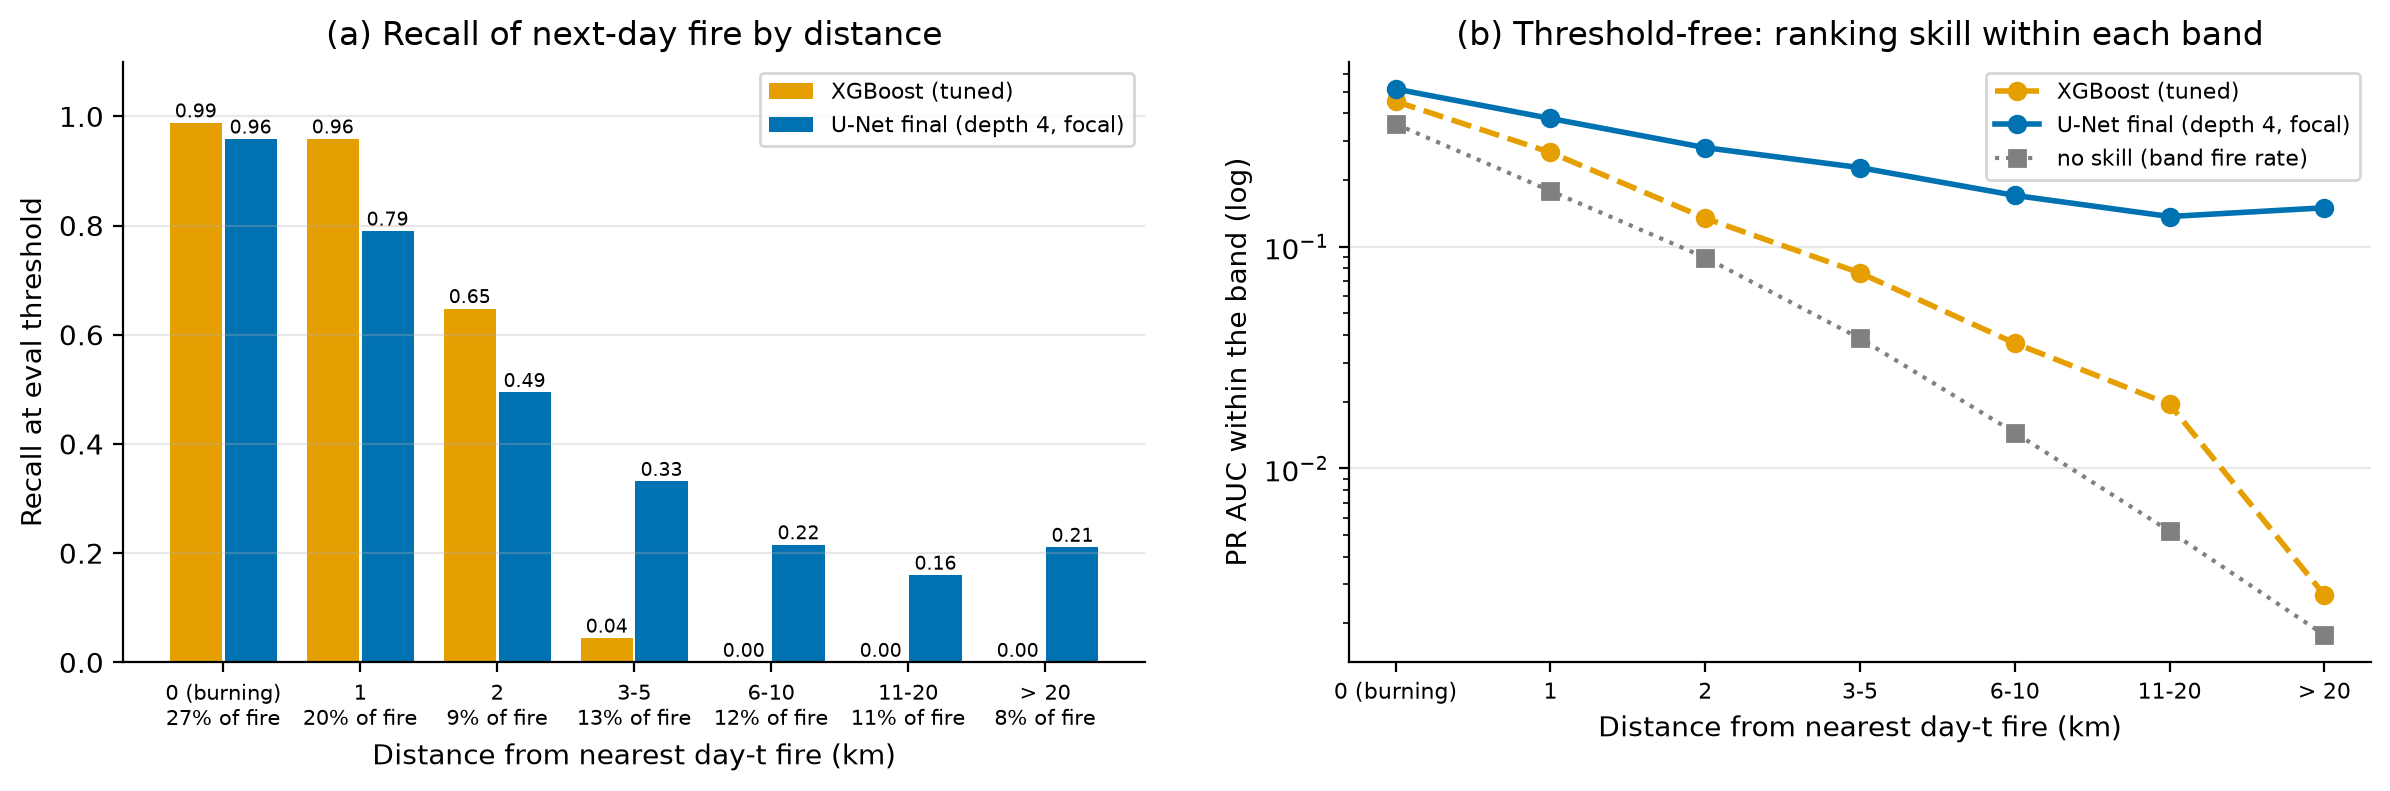
\includegraphics[width=\textwidth]{dl_eval_recall_by_distance.png}
\end{columns}
\src{Test split, seed 0 at eval-chosen thresholds; PR AUC over seeds 0--2. Notebook 03, sections 4 and 4b.}
\end{frame}

% ---------------------------------------------------------------- Sachin
\begin{frame}{Dying fires: fewer false alarms, still not recognised}
\begin{columns}[T]
\column{0.44\textwidth}
\footnotesize
\begin{itemize}
\item False positives \textbf{$-$22\%} (138.7k $\rightarrow$ 108.6k); $-$25\% around shrinking fires
\item Why: a tighter halo that follows the fire's shape
\item But it cannot tell which burning pixel goes out: ROC AUC 0.66 vs 0.65 for XGBoost
\item \textbf{Per fire event}: mean PR AUC \textbf{0.506} vs 0.187, better in 92\% of events; small fires 0.59 vs 0.16
\end{itemize}
\column{0.54\textwidth}
\centering
\vspace{0.3em}
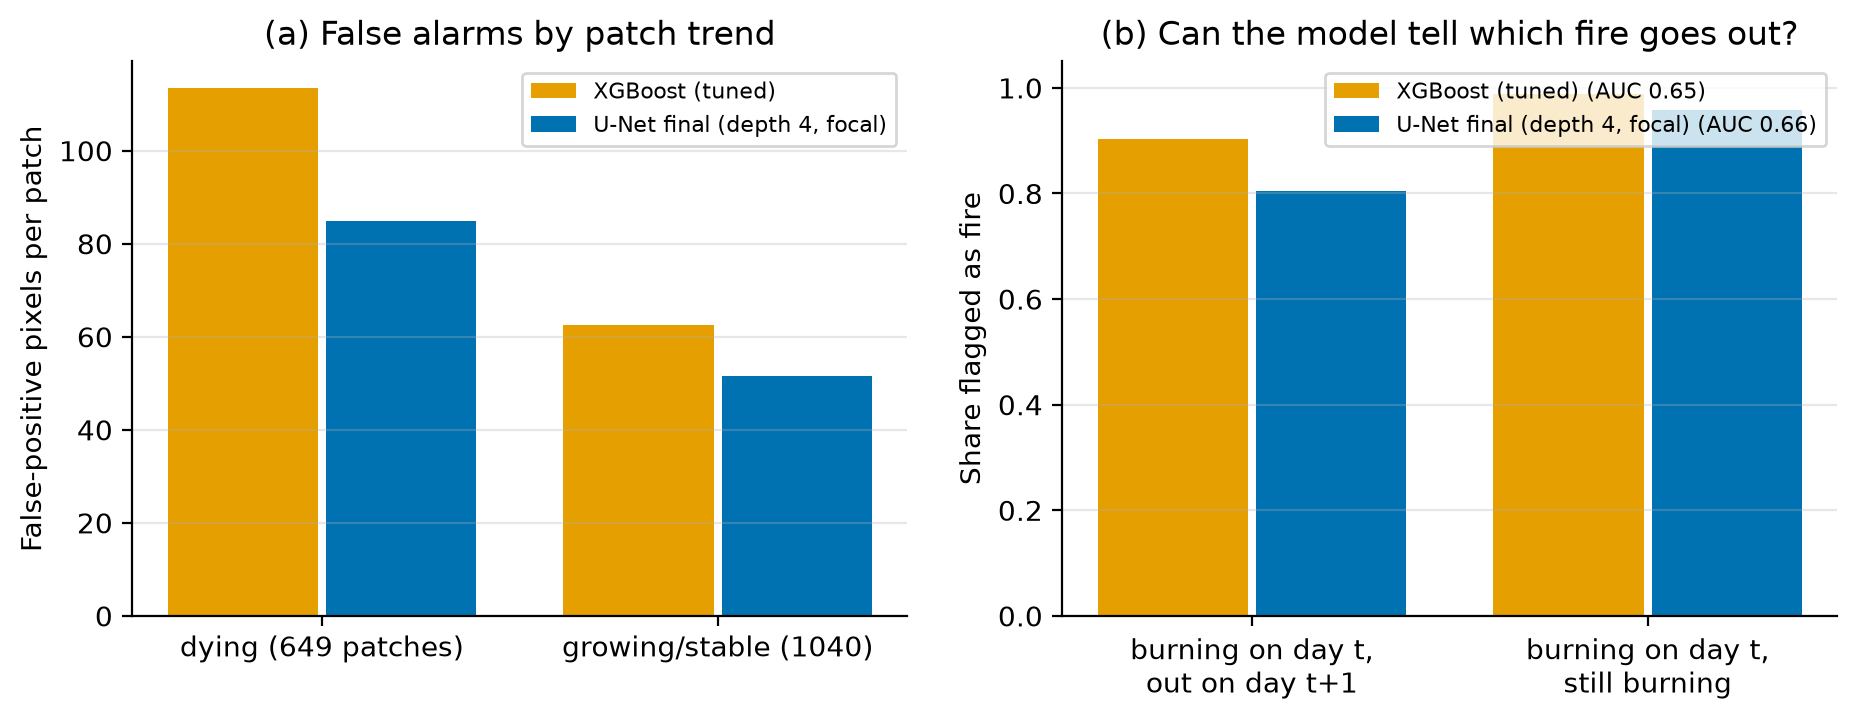
\includegraphics[width=\textwidth]{dl_eval_dying_fires.png}
\end{columns}
\src{Dying patch: fewer burning pixels on day $t{+}1$ than on day $t$ (649 of 1\,689). Notebook 03, sections 5 and 8.}
\end{frame}

% ---------------------------------------------------------------- Sachin
\begin{frame}{What the U-Net looks at: the fire front, not the wind}
\begin{columns}[T]
\column{0.40\textwidth}
\footnotesize
\begin{itemize}
\item Blanking today's fire: $-$0.171 PR AUC; every other group $\leq$ 0.013, as in Phase 1's SHAP
\item Saliency \textbf{5$\times$} the average on burning pixels, 4$\times$ at 1\,km: it reads the front
\item \textbf{Not plausible yet:} no downwind push (score ratio 1.01; data on train 1.1--3.1)
\item Both open errors need inputs one day lacks: burnt fuel, suppression, next-day weather
\end{itemize}
\column{0.58\textwidth}
\centering
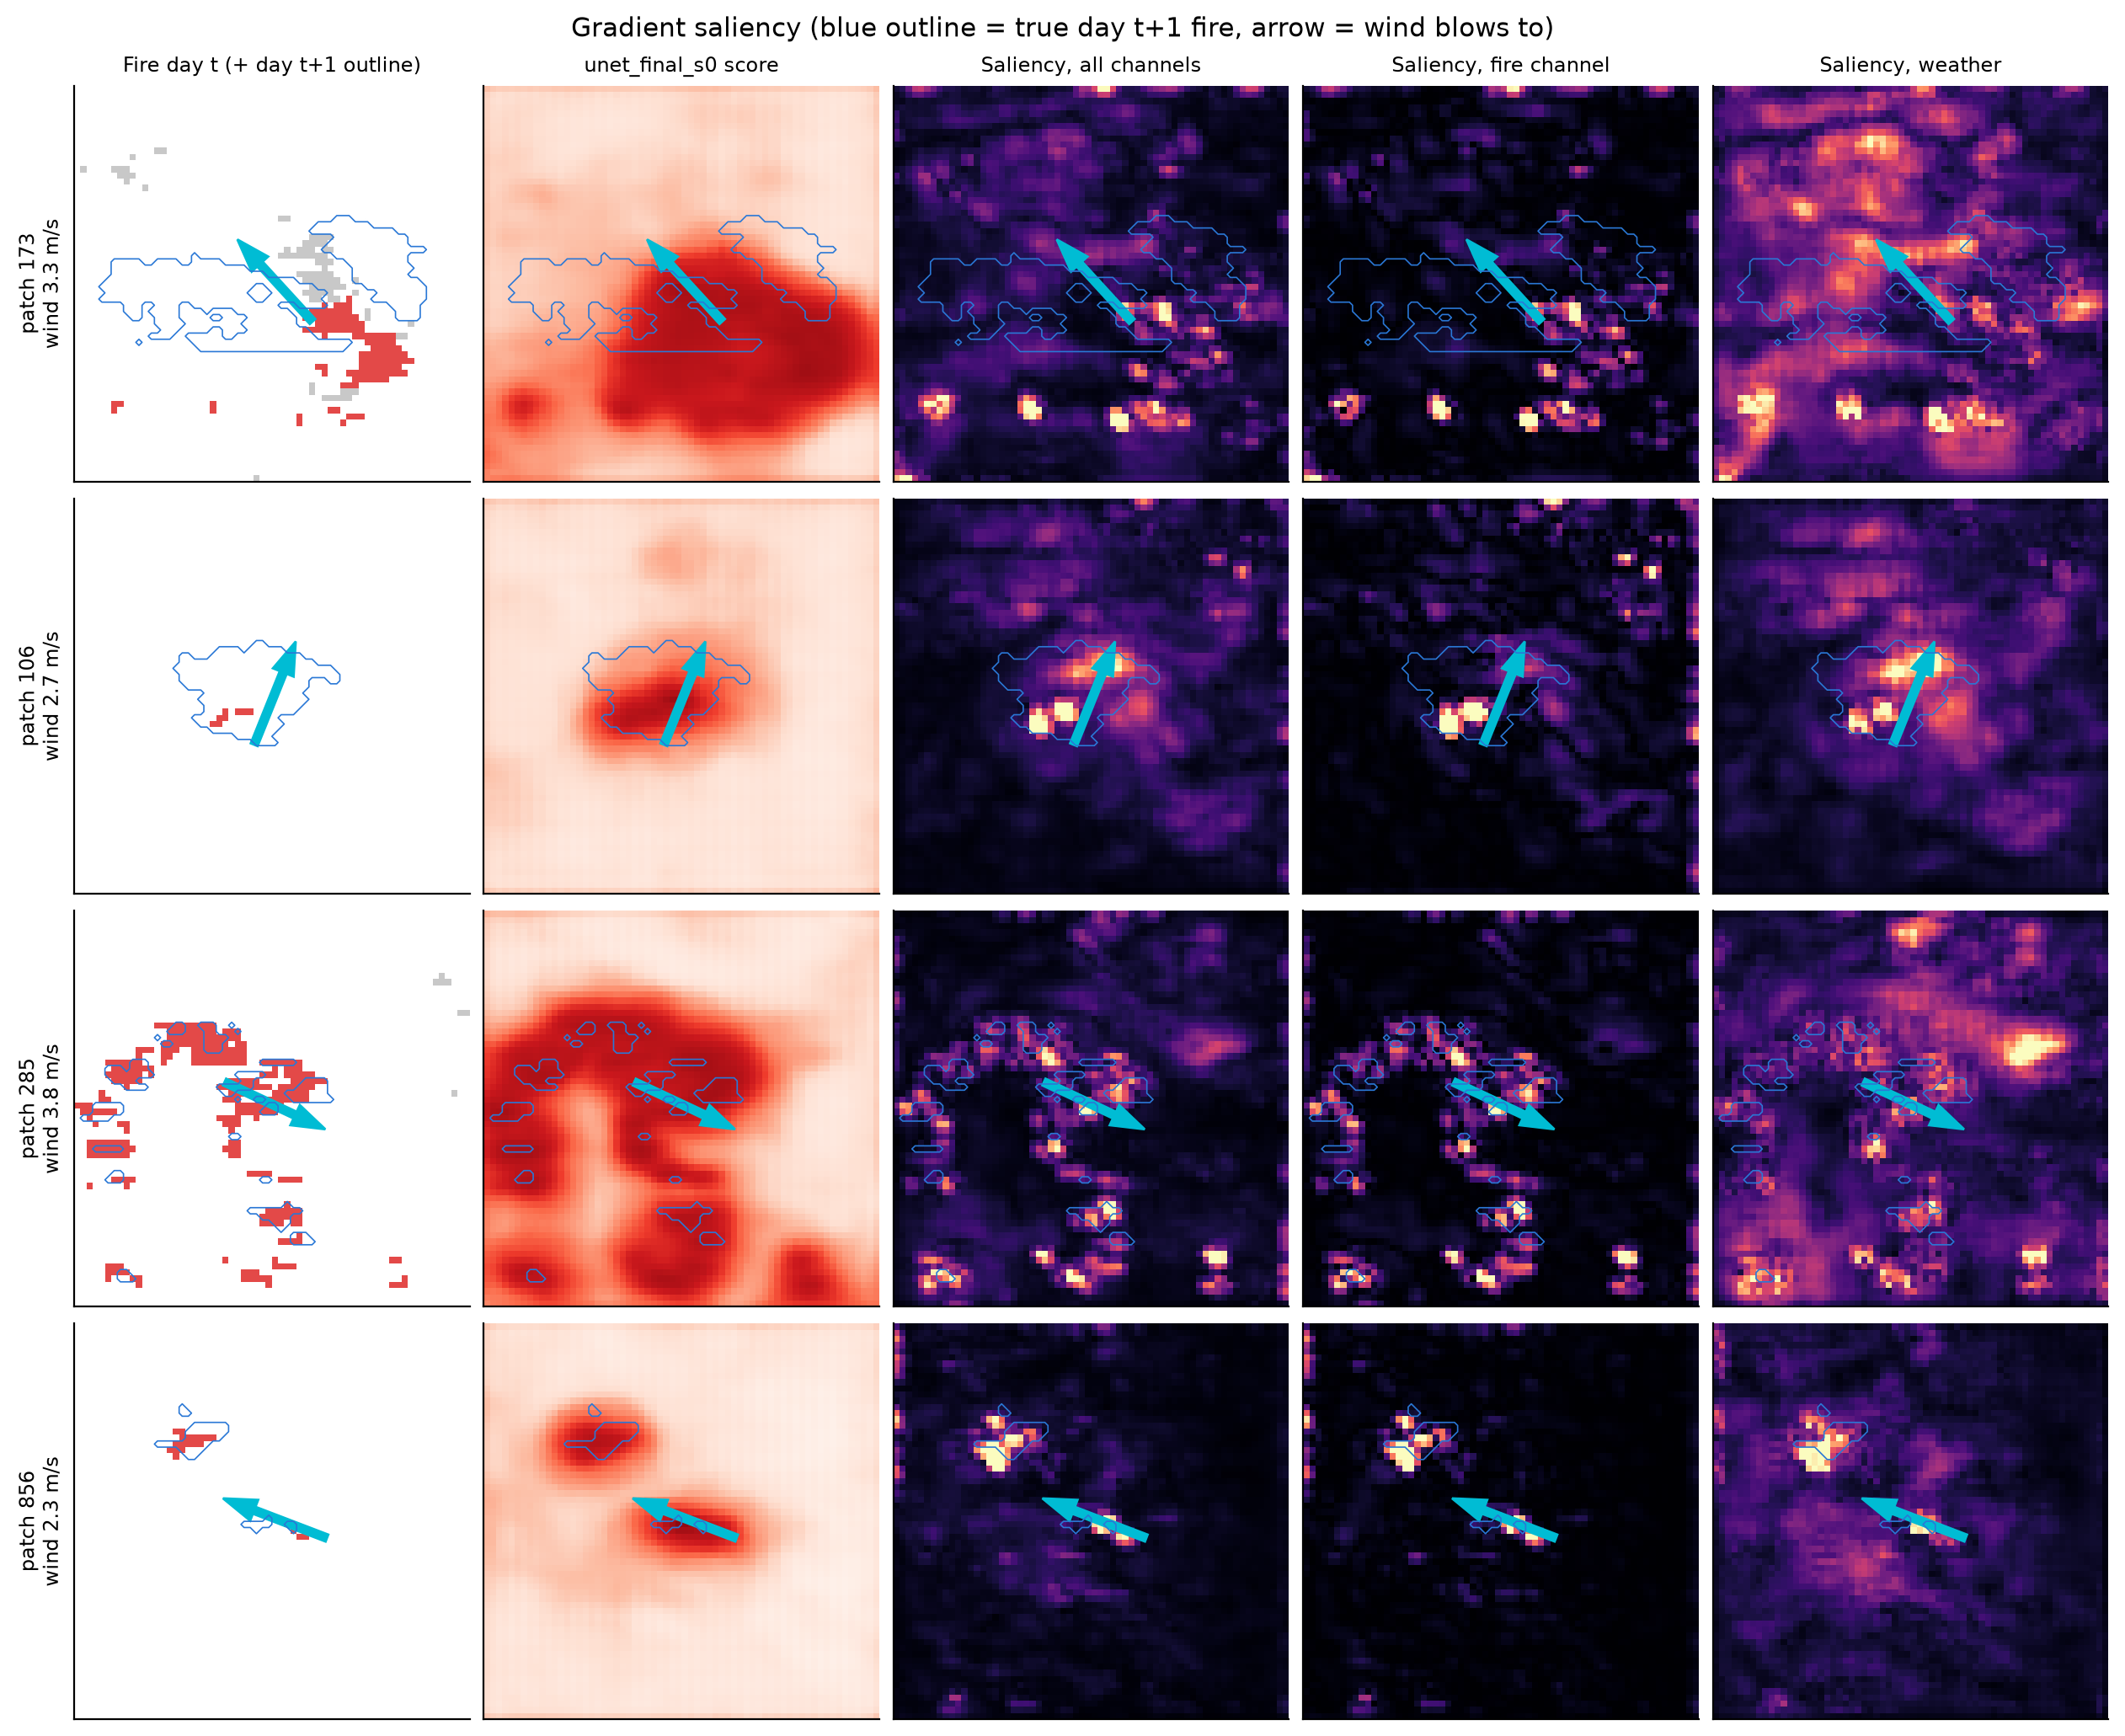
\includegraphics[height=0.70\textheight]{dl_eval_saliency_maps.png}
\end{columns}
\src{Gradient of each patch's predicted fire w.r.t. the inputs (final U-Net, seed 0). Notebook 03, sections 6 and 7.}
\end{frame}

% Suggested spot: after "Can we trust the U-Net?". They use the deck's \src command and graphicspath
% (../reports/dl/figures/). Numbers: notebooks/03_dl_evaluation.ipynb. Checked to compile without overflow.

% ---------------------------------------------------------------- Sachin
\begin{frame}{Phase 1 missed fire far from the front. The U-Net finds some}
\begin{columns}[T]
\column{0.44\textwidth}
\footnotesize
\begin{itemize}
\item Final U-Net (depth 4, focal): \textbf{0.344 $\pm$ 0.007} PR AUC vs 0.255 for XGBoost; paired over fire events +0.080 (0.058 to 0.113)
\item Fire \textbf{beyond 5\,km}: recall \textbf{0.20}, XGBoost \textbf{0.00}
\item 3--5\,km: 0.33 vs 0.04; ahead in every band
\item Not memorised places, not hidden fire, not a patch shortcut: stronger on unseen locations (0.18 vs 0.07)
\item Depth 4 is the step: depth 3 and the CNN only tie XGBoost
\end{itemize}
\column{0.54\textwidth}
\centering
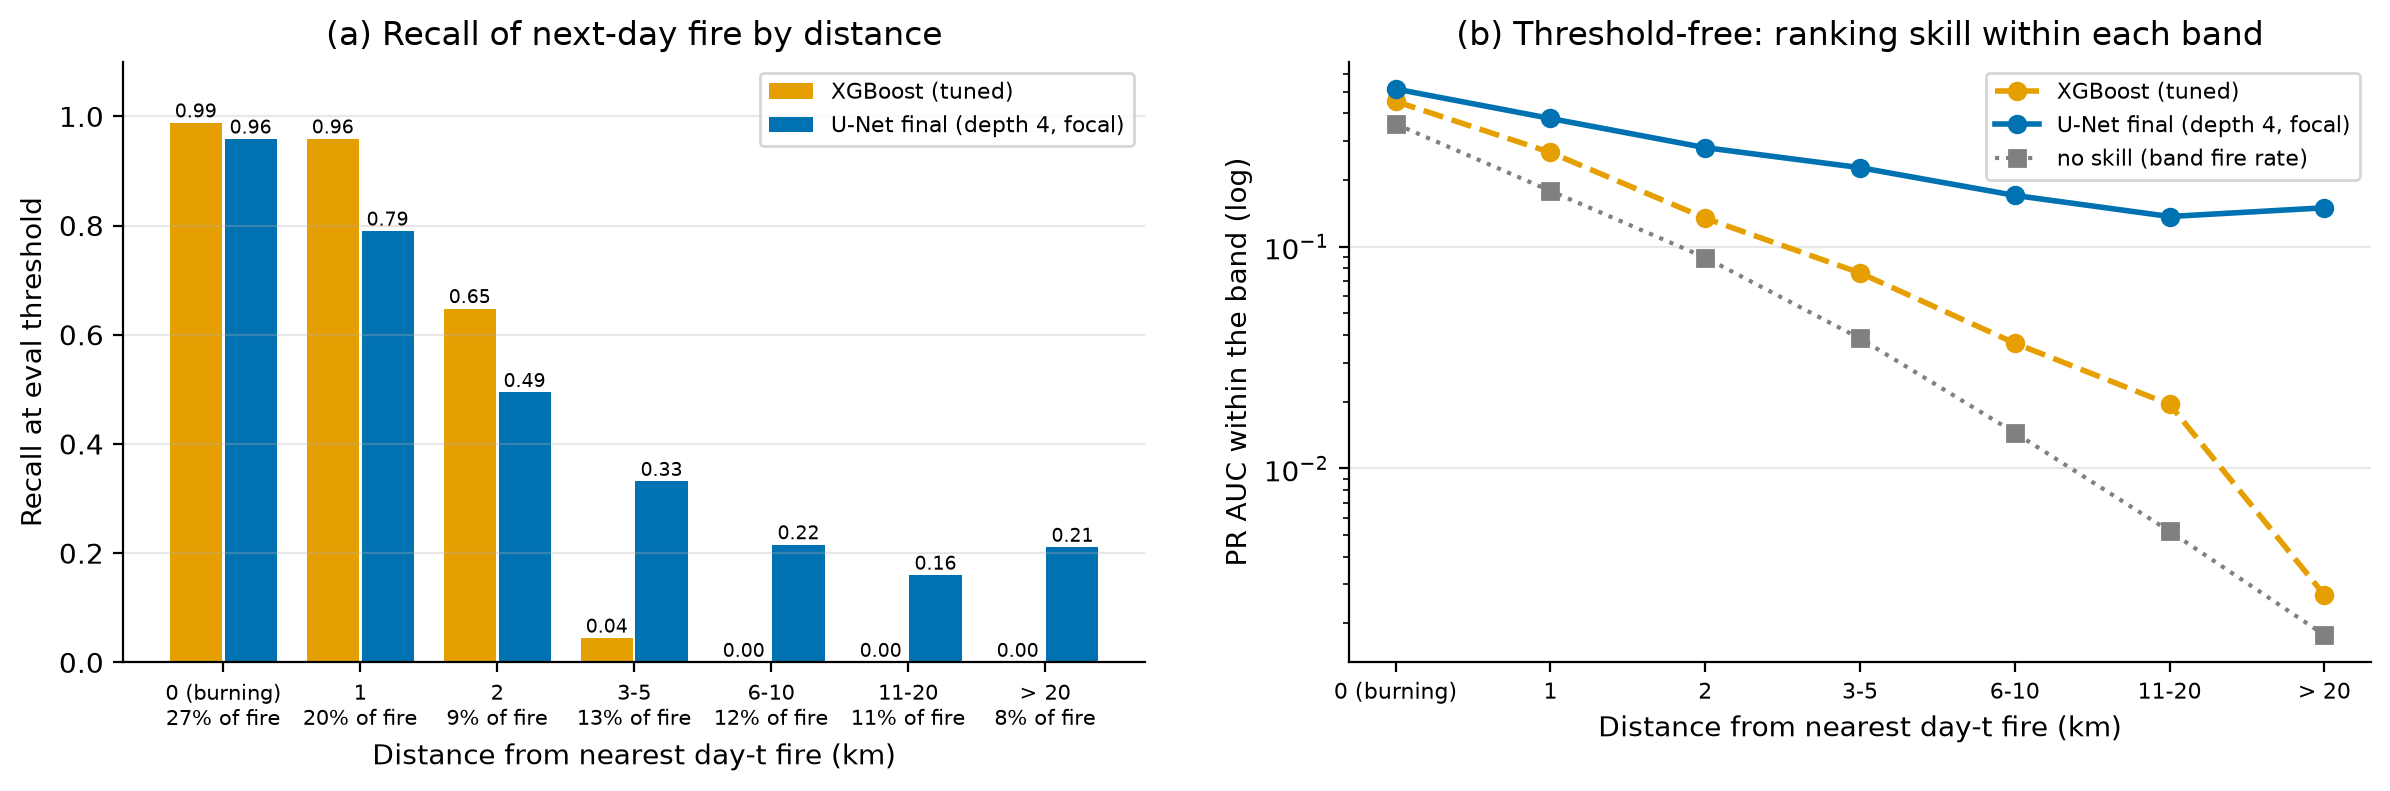
\includegraphics[width=\textwidth]{dl_eval_recall_by_distance.png}
\end{columns}
\src{Test split, seed 0 at eval-chosen thresholds; PR AUC over seeds 0--2. Notebook 03, sections 4 and 4b.}
\end{frame}

% ---------------------------------------------------------------- Sachin
\begin{frame}{Dying fires: fewer false alarms, still not recognised}
\begin{columns}[T]
\column{0.44\textwidth}
\footnotesize
\begin{itemize}
\item False positives \textbf{$-$22\%} (138.7k $\rightarrow$ 108.6k); $-$25\% around shrinking fires
\item Why: a tighter halo that follows the fire's shape
\item But it cannot tell which burning pixel goes out: ROC AUC 0.66 vs 0.65 for XGBoost
\item \textbf{Per fire event}: mean PR AUC \textbf{0.506} vs 0.187, better in 92\% of events; small fires 0.59 vs 0.16
\end{itemize}
\column{0.54\textwidth}
\centering
\vspace{0.3em}
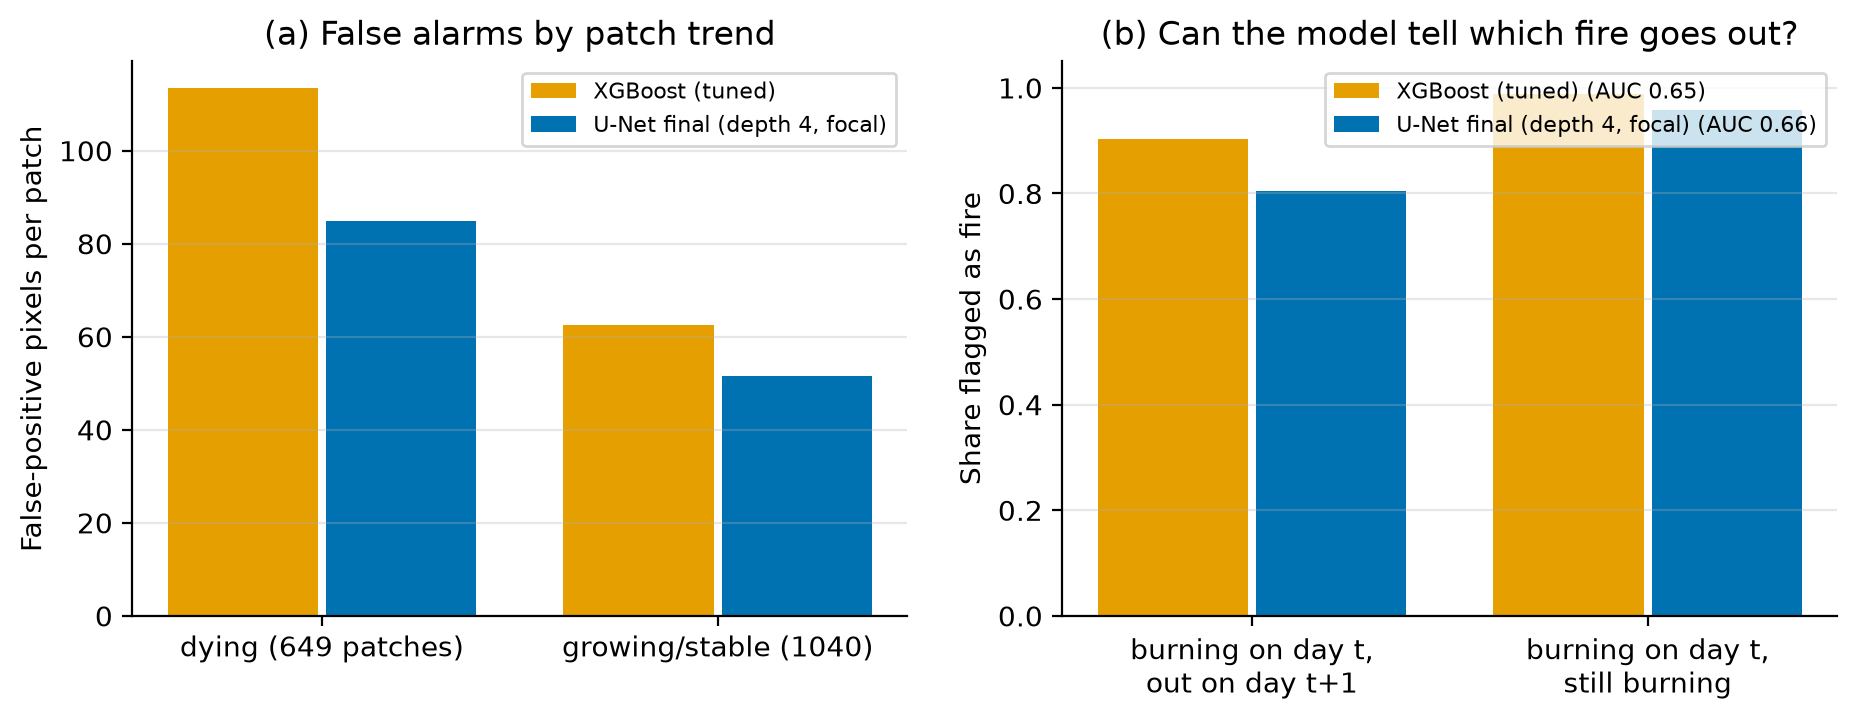
\includegraphics[width=\textwidth]{dl_eval_dying_fires.png}
\end{columns}
\src{Dying patch: fewer burning pixels on day $t{+}1$ than on day $t$ (649 of 1\,689). Notebook 03, sections 5 and 8.}
\end{frame}

% ---------------------------------------------------------------- Sachin
\begin{frame}{What the U-Net looks at: the fire front, not the wind}
\begin{columns}[T]
\column{0.40\textwidth}
\footnotesize
\begin{itemize}
\item Blanking today's fire: $-$0.171 PR AUC; every other group $\leq$ 0.013, as in Phase 1's SHAP
\item Saliency \textbf{5$\times$} the average on burning pixels, 4$\times$ at 1\,km: it reads the front
\item \textbf{Not plausible yet:} no downwind push (score ratio 1.01; data on train 1.1--3.1)
\item Both open errors need inputs one day lacks: burnt fuel, suppression, next-day weather
\end{itemize}
\column{0.58\textwidth}
\centering
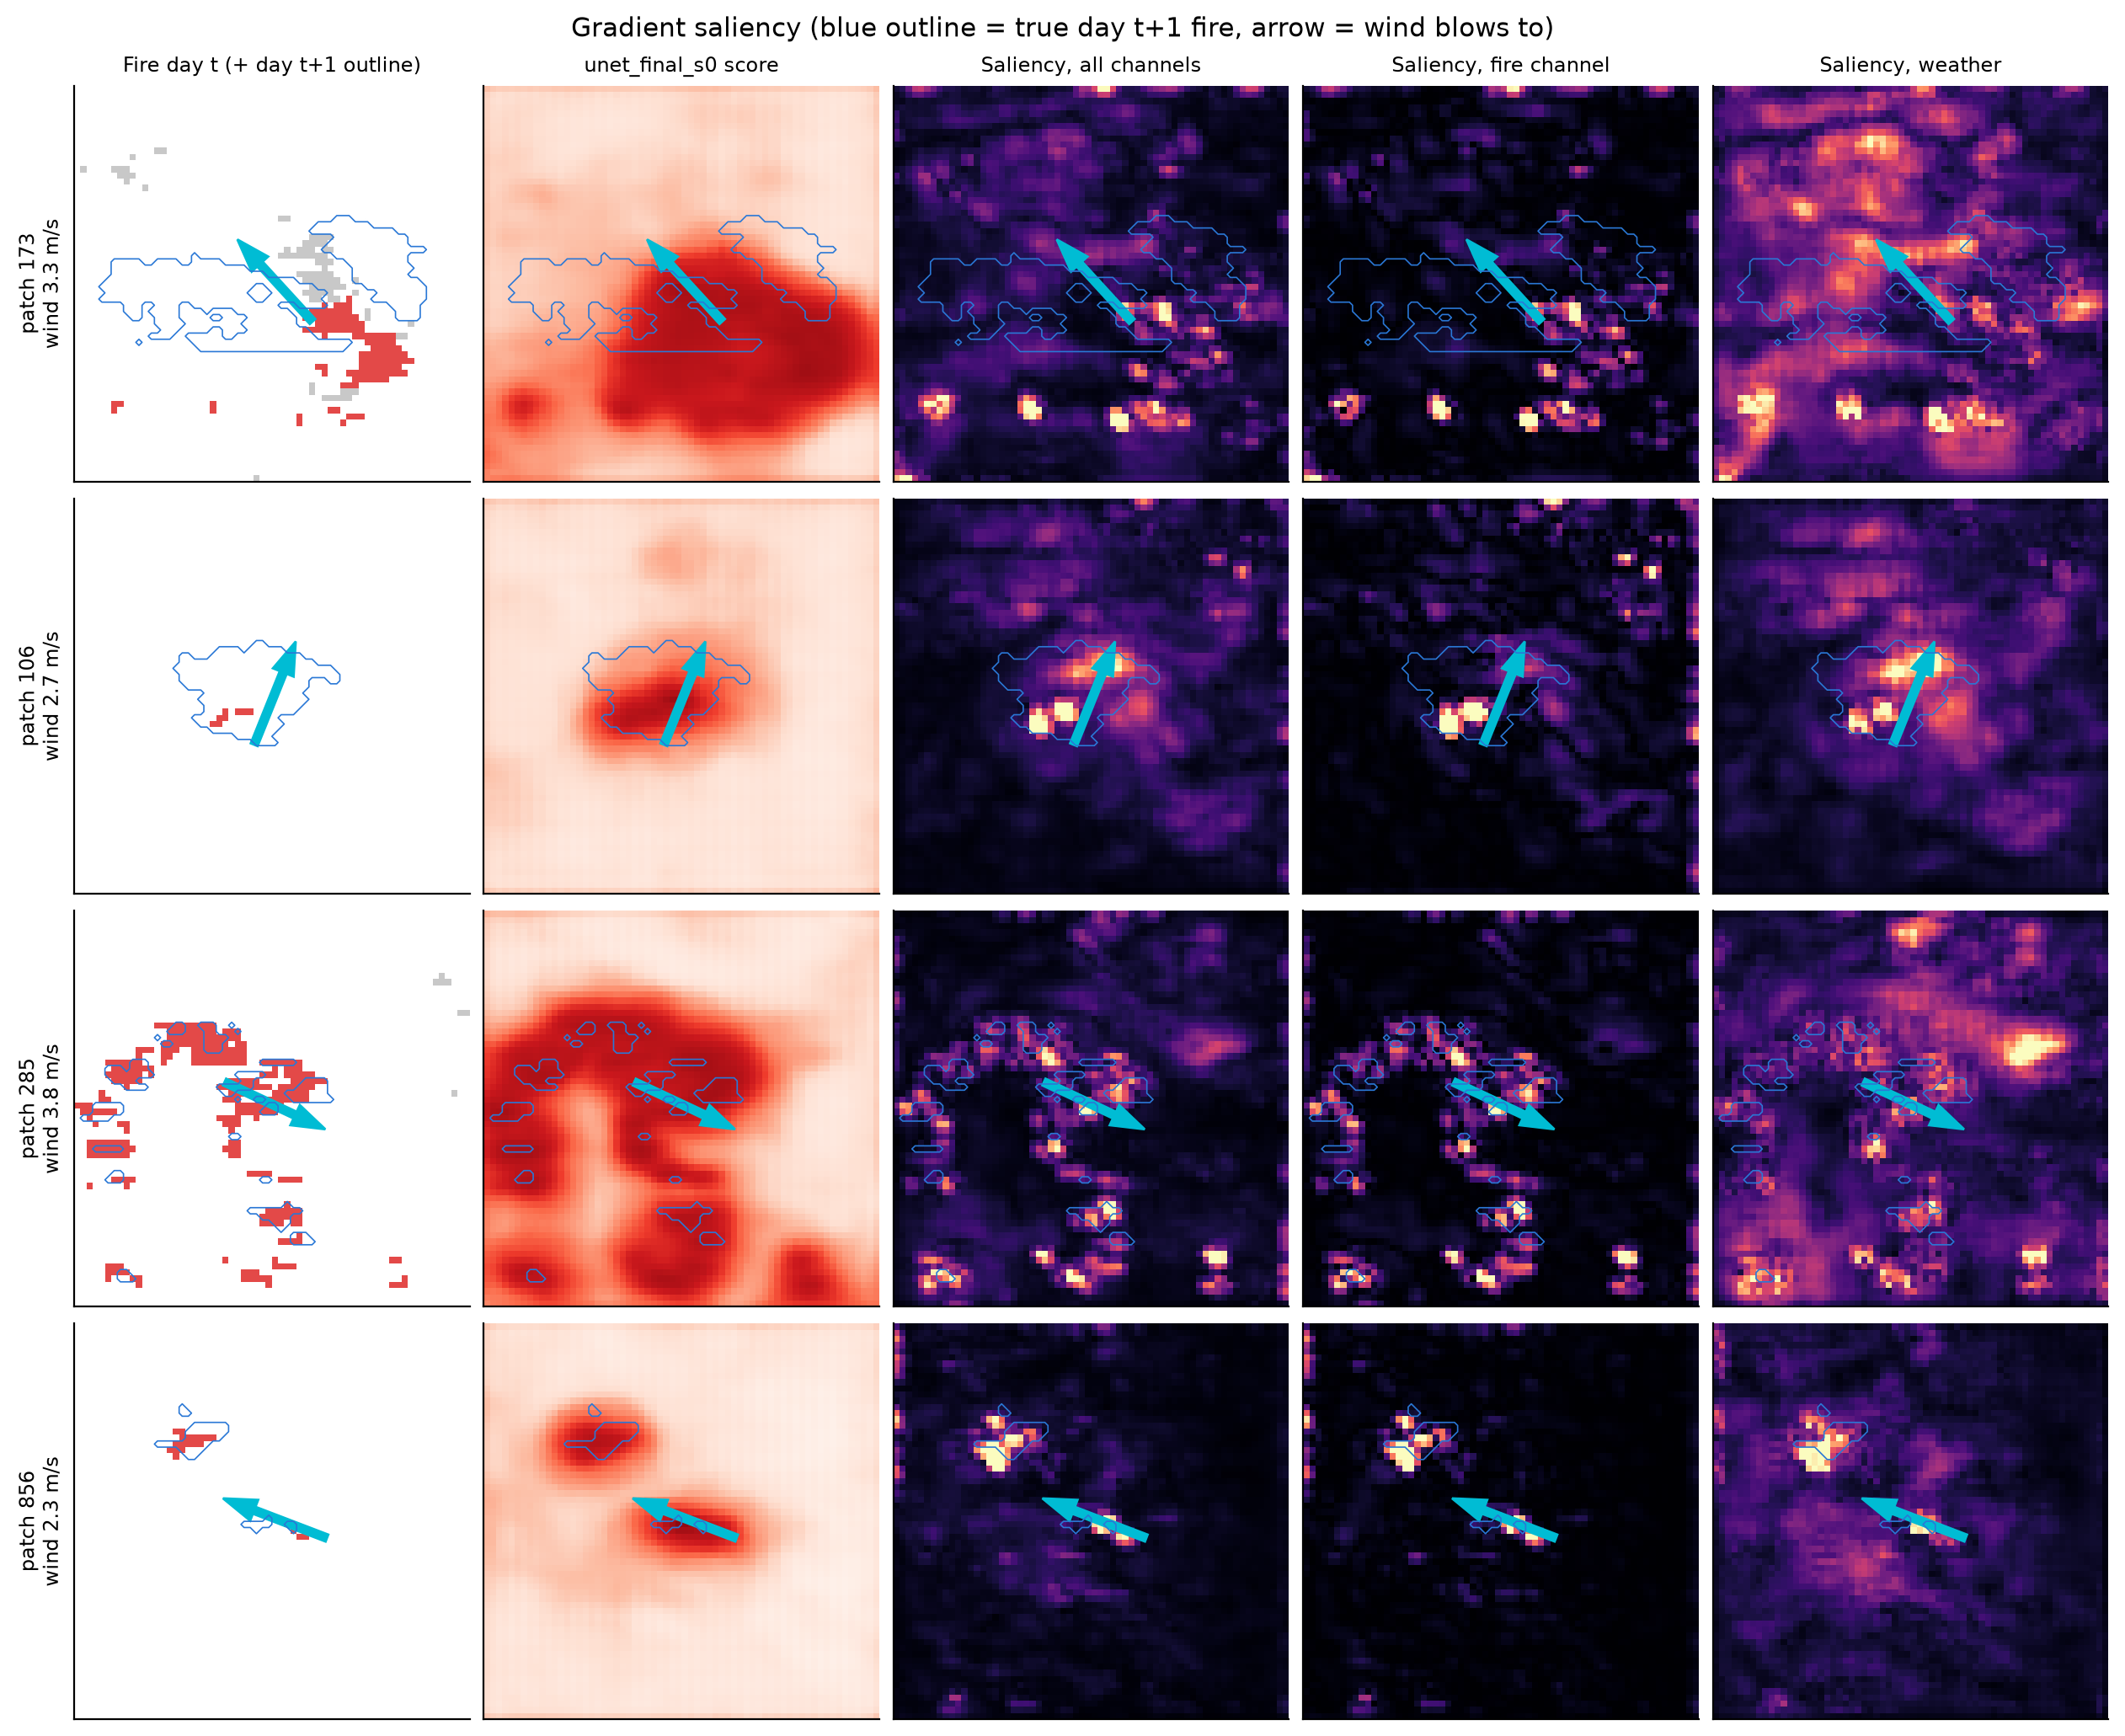
\includegraphics[height=0.70\textheight]{dl_eval_saliency_maps.png}
\end{columns}
\src{Gradient of each patch's predicted fire w.r.t. the inputs (final U-Net, seed 0). Notebook 03, sections 6 and 7.}
\end{frame}

% Suggested spot: after "Can we trust the U-Net?". They use the deck's \src command and graphicspath
% (../reports/dl/figures/). Numbers: notebooks/03_dl_evaluation.ipynb. Checked to compile without overflow.

% ---------------------------------------------------------------- Sachin
\begin{frame}{Phase 1 missed fire far from the front. The U-Net finds some}
\begin{columns}[T]
\column{0.44\textwidth}
\footnotesize
\begin{itemize}
\item Final U-Net (depth 4, focal): \textbf{0.344 $\pm$ 0.007} PR AUC vs 0.255 for XGBoost; paired over fire events +0.080 (0.058 to 0.113)
\item Fire \textbf{beyond 5\,km}: recall \textbf{0.20}, XGBoost \textbf{0.00}
\item 3--5\,km: 0.33 vs 0.04; ahead in every band
\item Not memorised places, not hidden fire, not a patch shortcut: stronger on unseen locations (0.18 vs 0.07)
\item Depth 4 is the step: depth 3 and the CNN only tie XGBoost
\end{itemize}
\column{0.54\textwidth}
\centering
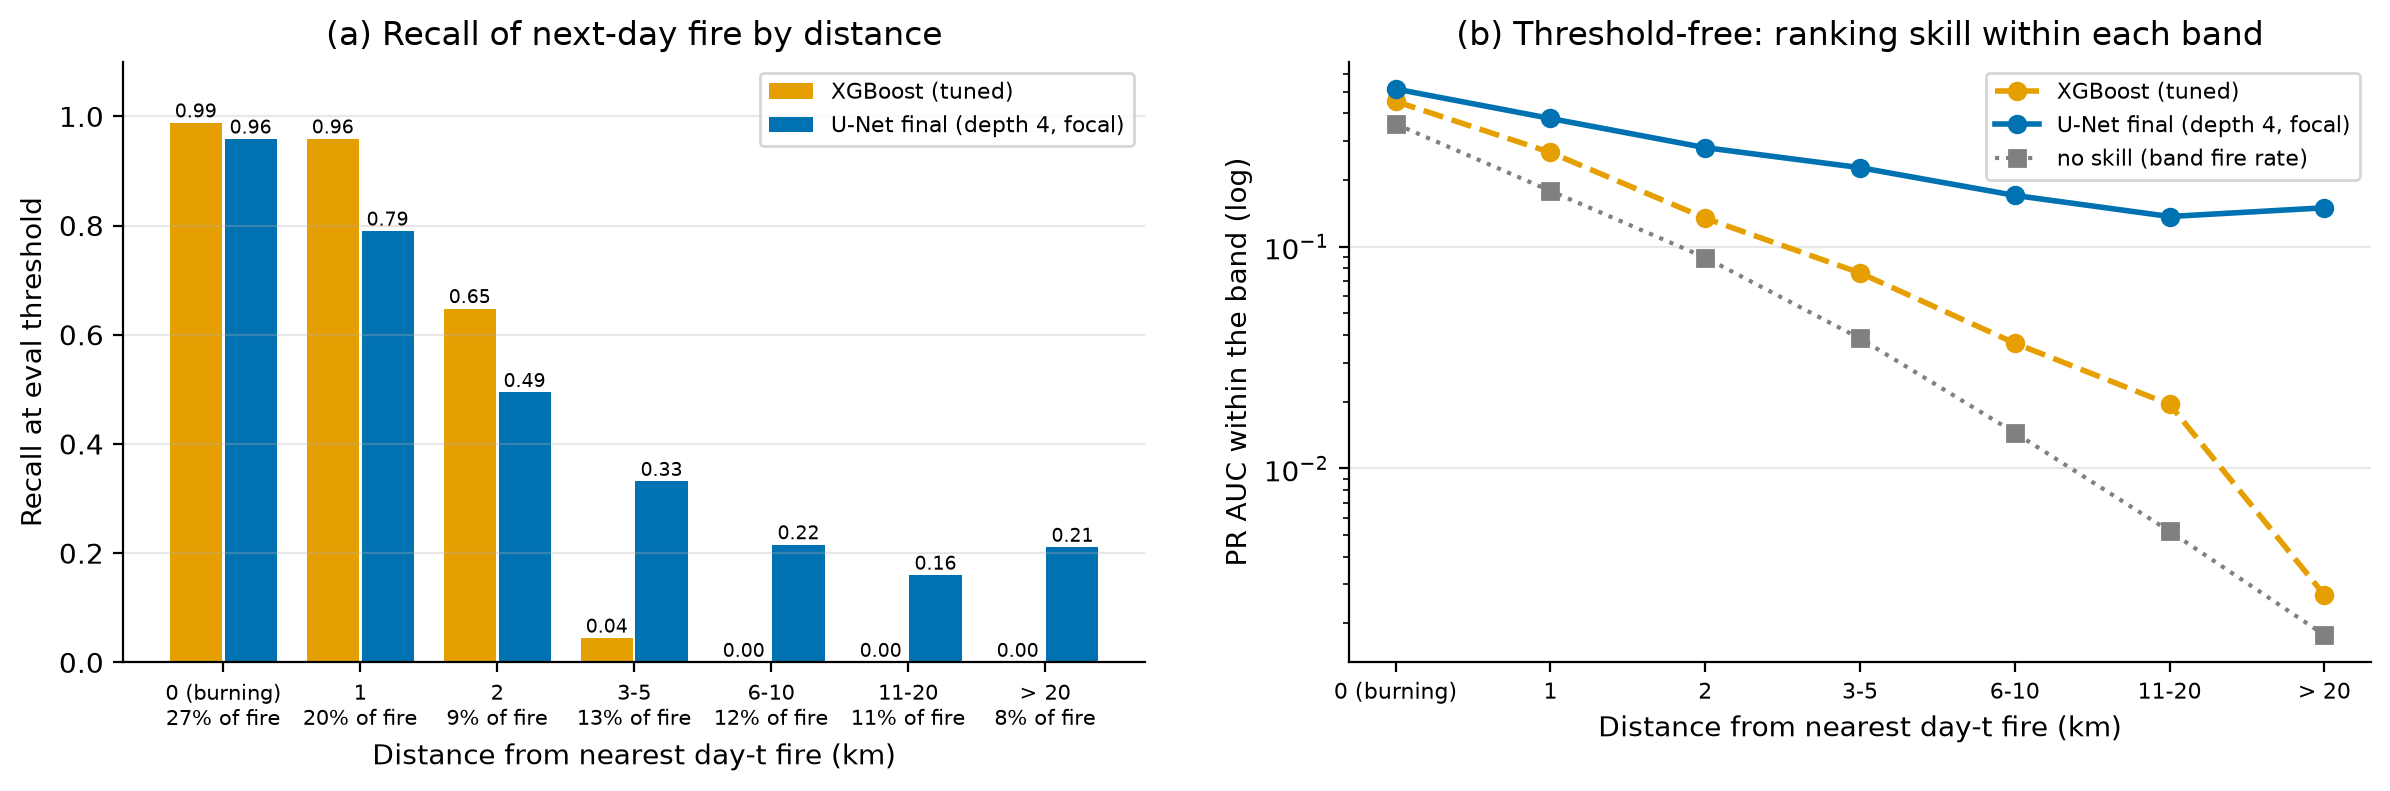
\includegraphics[width=\textwidth]{dl_eval_recall_by_distance.png}
\end{columns}
\src{Test split, seed 0 at eval-chosen thresholds; PR AUC over seeds 0--2. Notebook 03, sections 4 and 4b.}
\end{frame}

% ---------------------------------------------------------------- Sachin
\begin{frame}{Dying fires: fewer false alarms, still not recognised}
\begin{columns}[T]
\column{0.44\textwidth}
\footnotesize
\begin{itemize}
\item False positives \textbf{$-$22\%} (138.7k $\rightarrow$ 108.6k); $-$25\% around shrinking fires
\item Why: a tighter halo that follows the fire's shape
\item But it cannot tell which burning pixel goes out: ROC AUC 0.66 vs 0.65 for XGBoost
\item \textbf{Per fire event}: mean PR AUC \textbf{0.506} vs 0.187, better in 92\% of events; small fires 0.59 vs 0.16
\end{itemize}
\column{0.54\textwidth}
\centering
\vspace{0.3em}
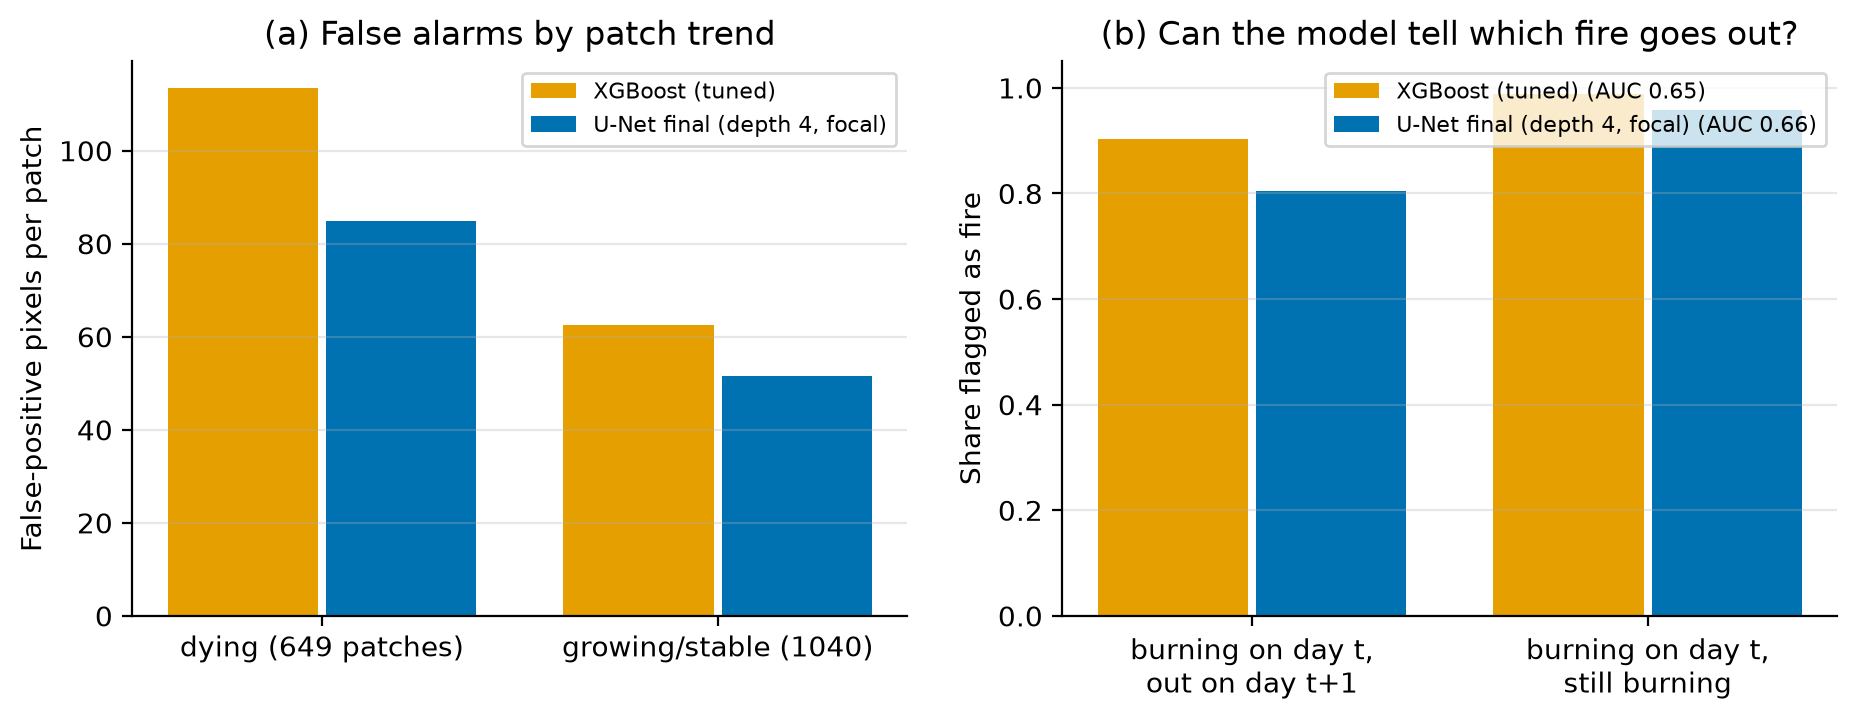
\includegraphics[width=\textwidth]{dl_eval_dying_fires.png}
\end{columns}
\src{Dying patch: fewer burning pixels on day $t{+}1$ than on day $t$ (649 of 1\,689). Notebook 03, sections 5 and 8.}
\end{frame}

% ---------------------------------------------------------------- Sachin
\begin{frame}{What the U-Net looks at: the fire front, not the wind}
\begin{columns}[T]
\column{0.40\textwidth}
\footnotesize
\begin{itemize}
\item Blanking today's fire: $-$0.171 PR AUC; every other group $\leq$ 0.013, as in Phase 1's SHAP
\item Saliency \textbf{5$\times$} the average on burning pixels, 4$\times$ at 1\,km: it reads the front
\item \textbf{Not plausible yet:} no downwind push (score ratio 1.01; data on train 1.1--3.1)
\item Both open errors need inputs one day lacks: burnt fuel, suppression, next-day weather
\end{itemize}
\column{0.58\textwidth}
\centering
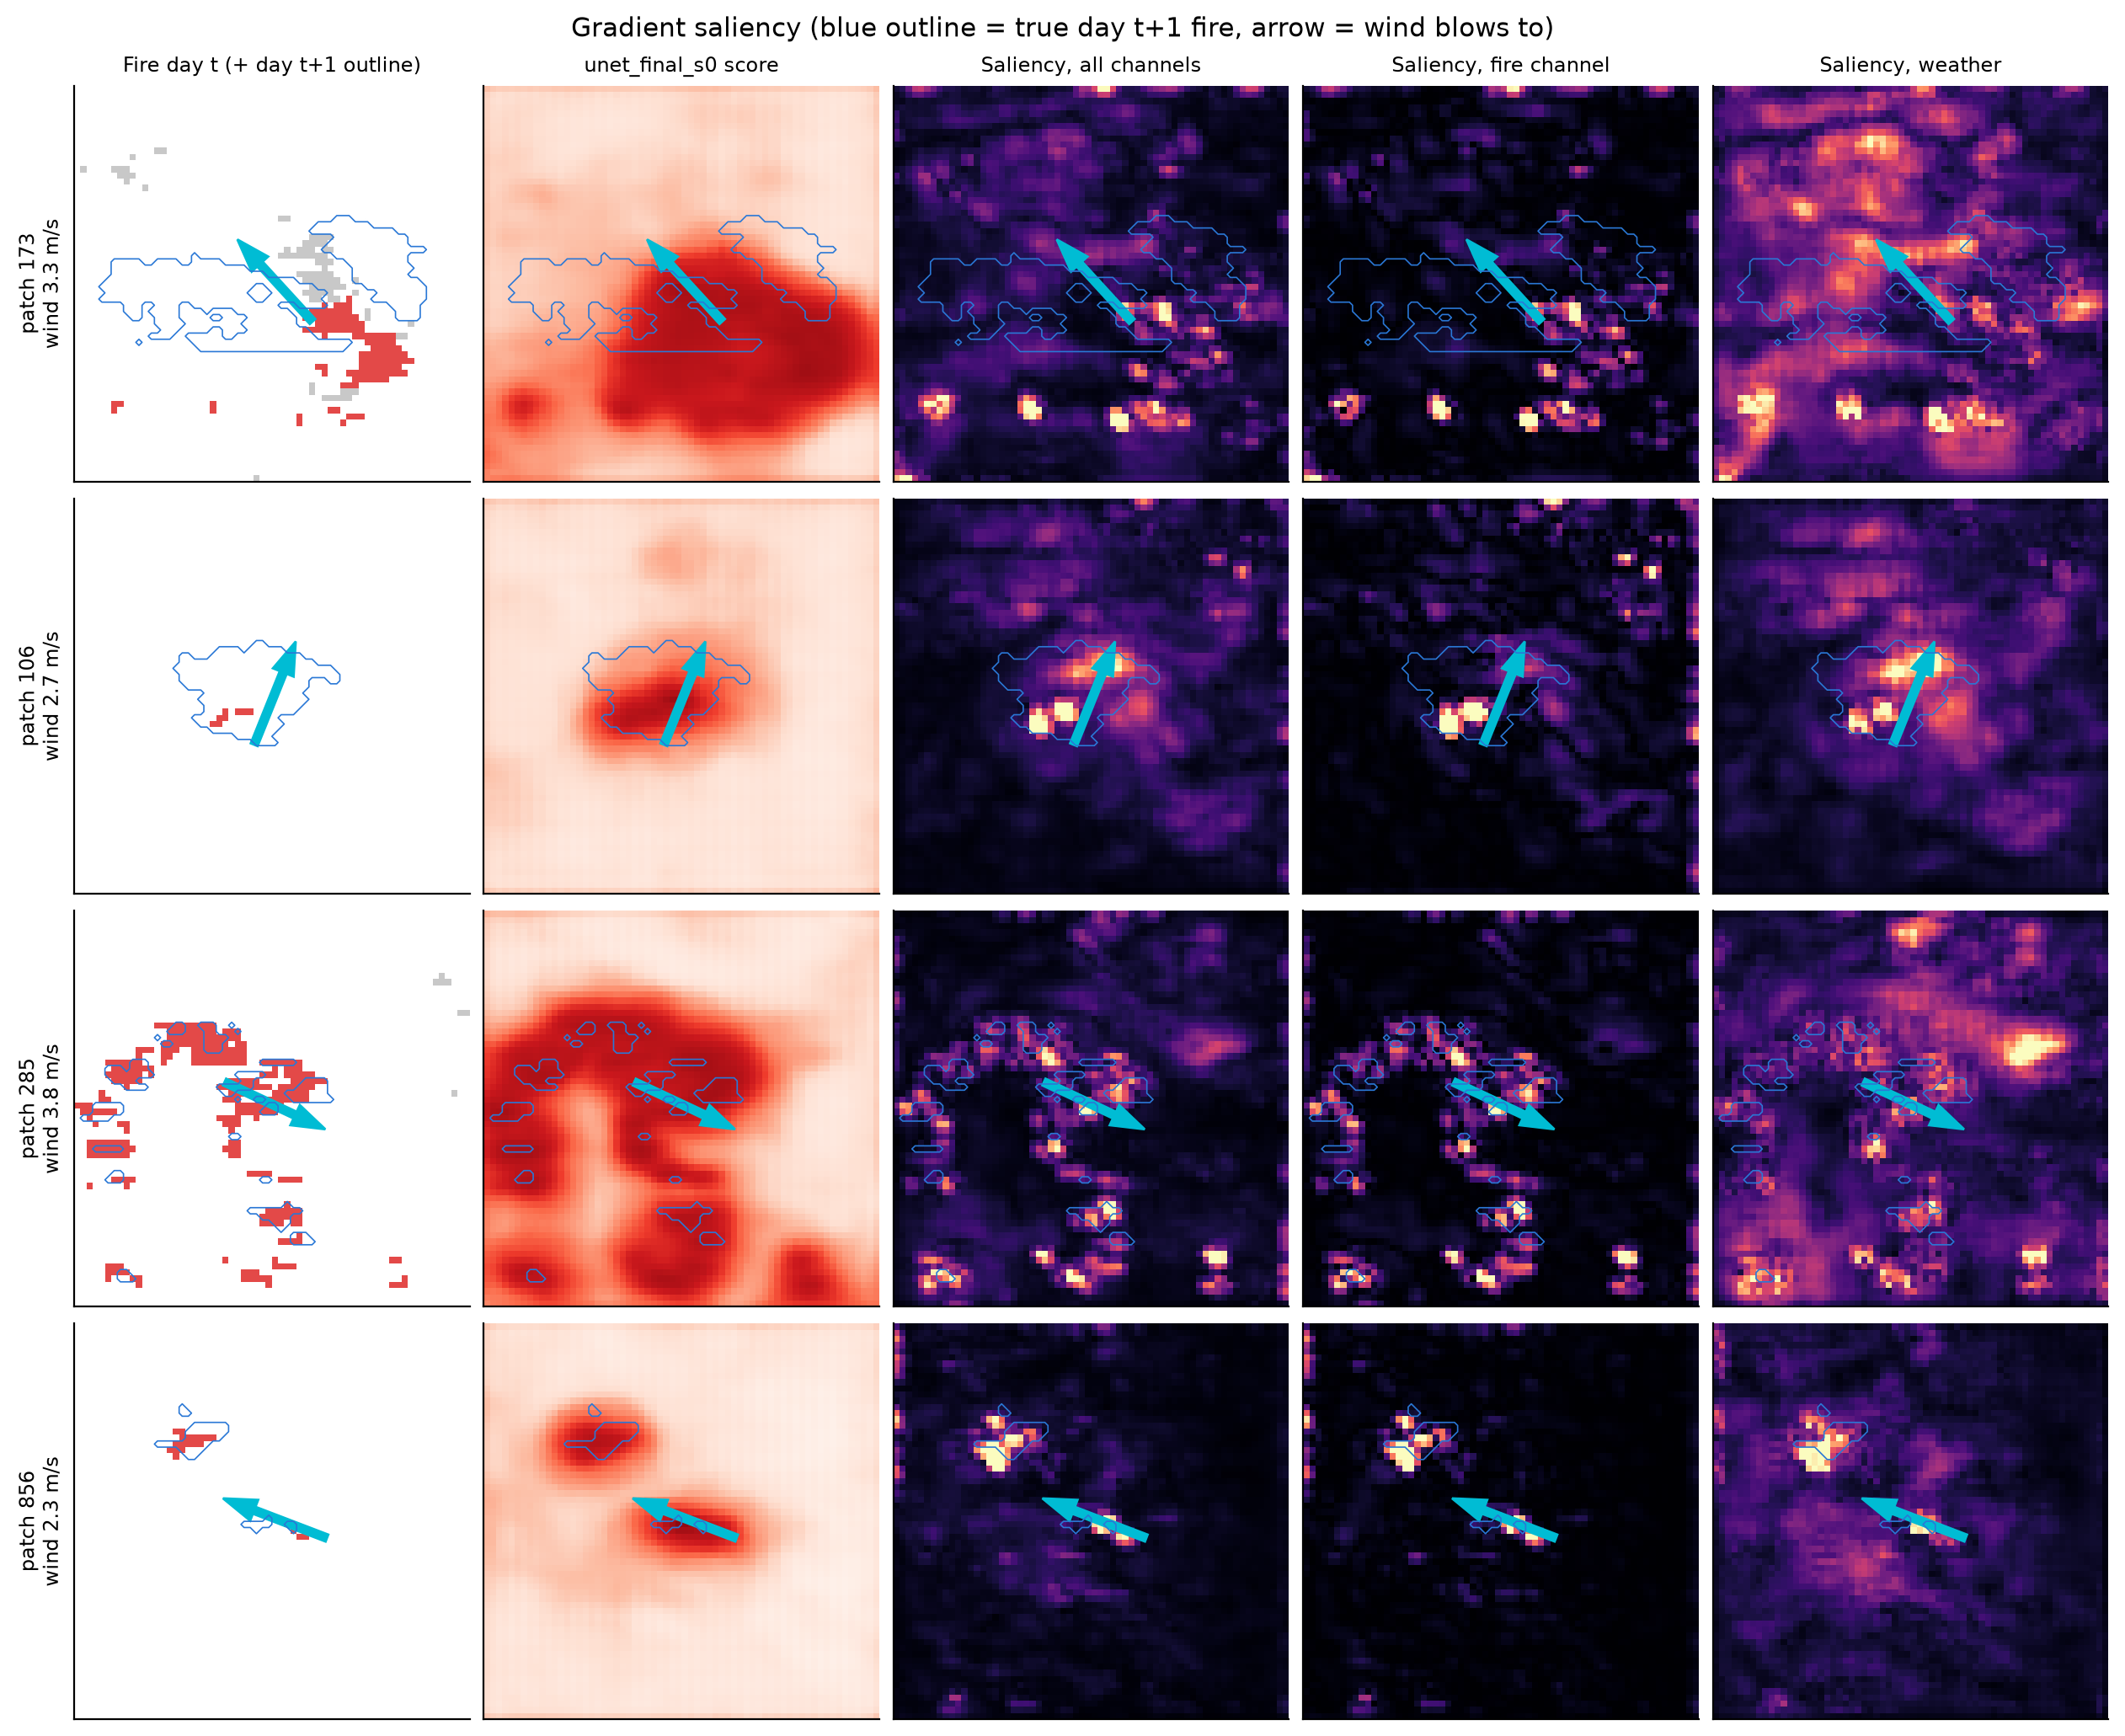
\includegraphics[height=0.70\textheight]{dl_eval_saliency_maps.png}
\end{columns}
\src{Gradient of each patch's predicted fire w.r.t. the inputs (final U-Net, seed 0). Notebook 03, sections 6 and 7.}
\end{frame}

% Suggested spot: after "Can we trust the U-Net?". They use the deck's \src command and graphicspath
% (../reports/dl/figures/). Numbers: notebooks/03_dl_evaluation.ipynb. Checked to compile without overflow.

% ---------------------------------------------------------------- Sachin
\begin{frame}{Phase 1 missed fire far from the front. The U-Net finds some}
\begin{columns}[T]
\column{0.44\textwidth}
\footnotesize
\begin{itemize}
\item Final U-Net (depth 4, focal): \textbf{0.344 $\pm$ 0.007} PR AUC vs 0.255 for XGBoost; paired over fire events +0.080 (0.058 to 0.113)
\item Fire \textbf{beyond 5\,km}: recall \textbf{0.20}, XGBoost \textbf{0.00}
\item 3--5\,km: 0.33 vs 0.04; ahead in every band
\item Not memorised places, not hidden fire, not a patch shortcut: stronger on unseen locations (0.18 vs 0.07)
\item Depth 4 is the step: depth 3 and the CNN only tie XGBoost
\end{itemize}
\column{0.54\textwidth}
\centering
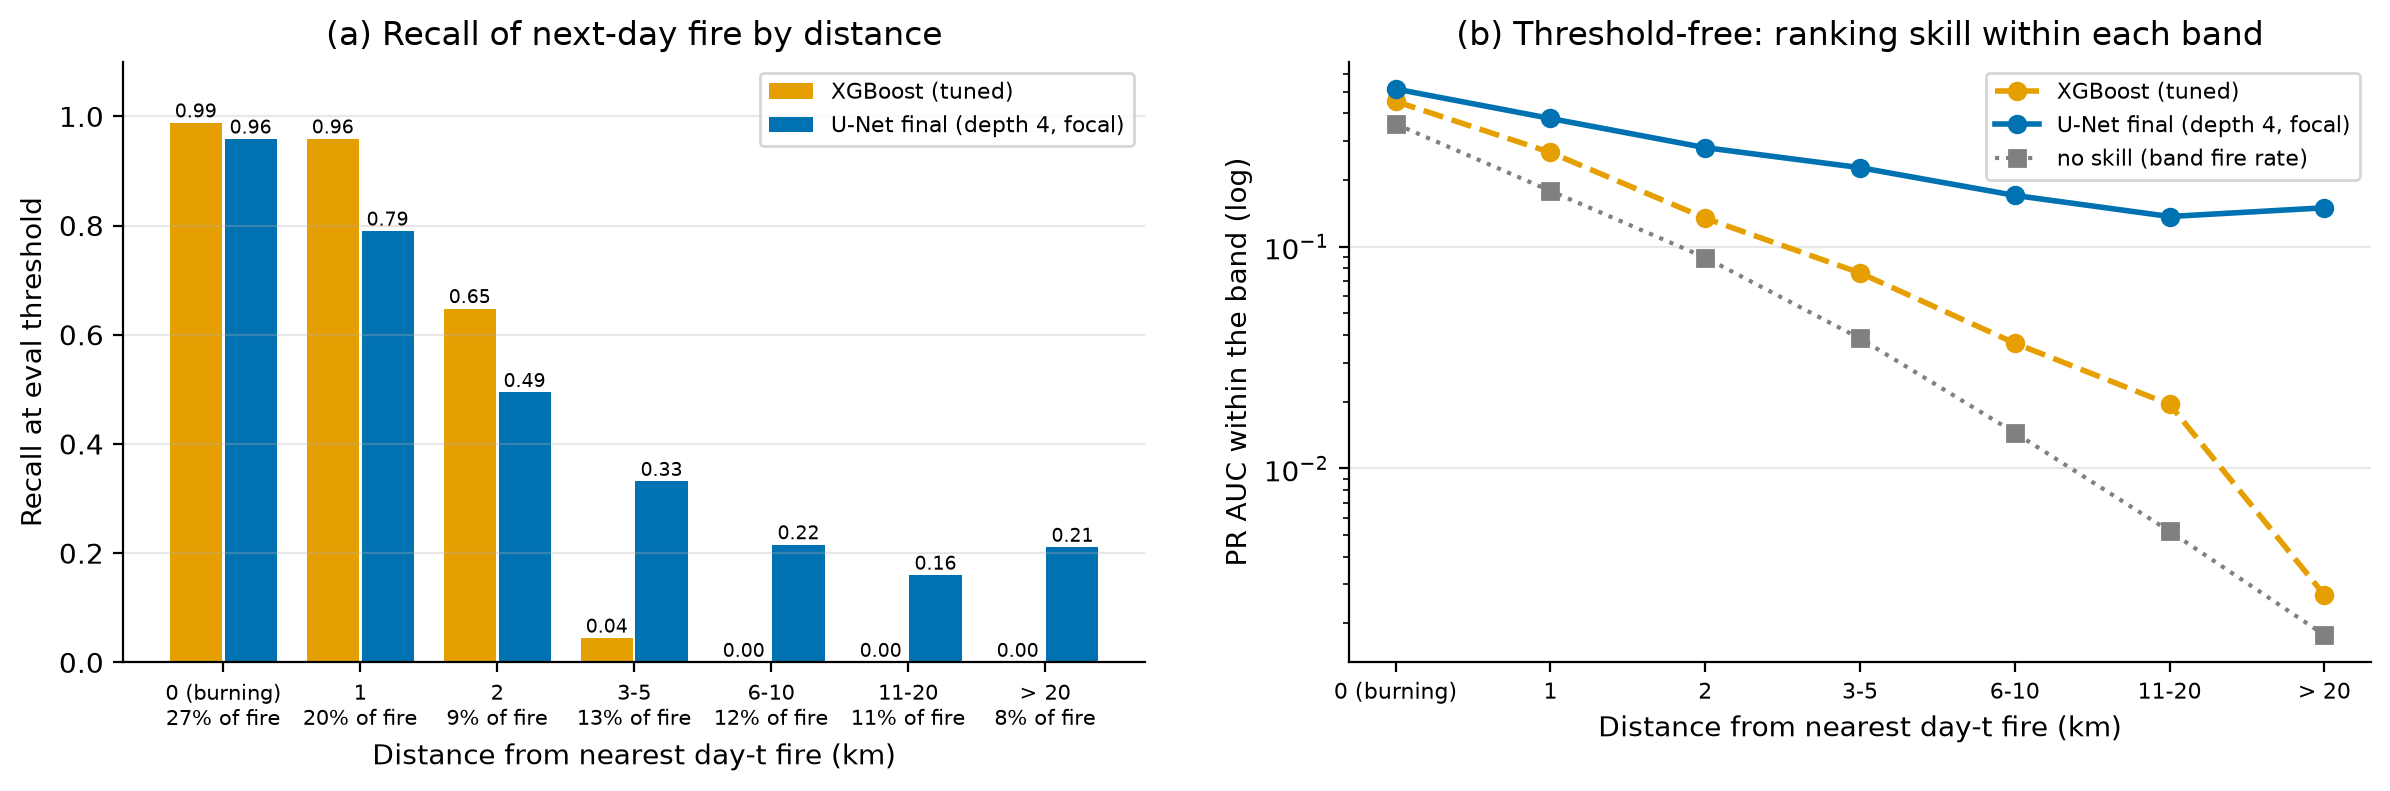
\includegraphics[width=\textwidth]{dl_eval_recall_by_distance.png}
\end{columns}
\src{Test split, seed 0 at eval-chosen thresholds; PR AUC over seeds 0--2. Notebook 03, sections 4 and 4b.}
\end{frame}

% ---------------------------------------------------------------- Sachin
\begin{frame}{Dying fires: fewer false alarms, still not recognised}
\begin{columns}[T]
\column{0.44\textwidth}
\footnotesize
\begin{itemize}
\item False positives \textbf{$-$22\%} (138.7k $\rightarrow$ 108.6k); $-$25\% around shrinking fires
\item Why: a tighter halo that follows the fire's shape
\item But it cannot tell which burning pixel goes out: ROC AUC 0.66 vs 0.65 for XGBoost
\item \textbf{Per fire event}: mean PR AUC \textbf{0.506} vs 0.187, better in 92\% of events; small fires 0.59 vs 0.16
\end{itemize}
\column{0.54\textwidth}
\centering
\vspace{0.3em}
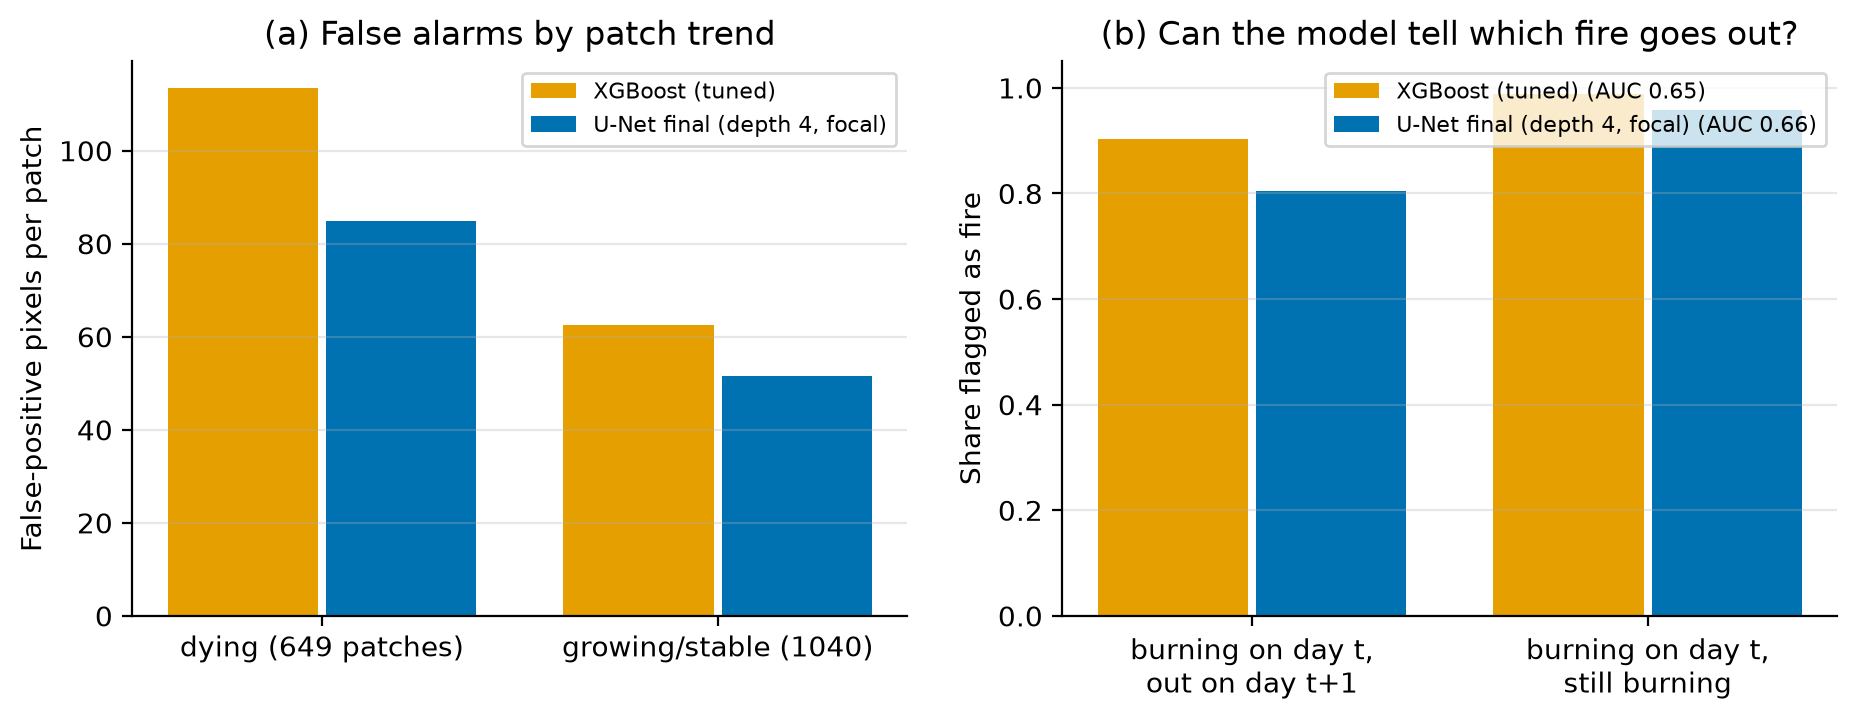
\includegraphics[width=\textwidth]{dl_eval_dying_fires.png}
\end{columns}
\src{Dying patch: fewer burning pixels on day $t{+}1$ than on day $t$ (649 of 1\,689). Notebook 03, sections 5 and 8.}
\end{frame}

% ---------------------------------------------------------------- Sachin
\begin{frame}{What the U-Net looks at: the fire front, not the wind}
\begin{columns}[T]
\column{0.40\textwidth}
\footnotesize
\begin{itemize}
\item Blanking today's fire: $-$0.171 PR AUC; every other group $\leq$ 0.013, as in Phase 1's SHAP
\item Saliency \textbf{5$\times$} the average on burning pixels, 4$\times$ at 1\,km: it reads the front
\item \textbf{Not plausible yet:} no downwind push (score ratio 1.01; data on train 1.1--3.1)
\item Both open errors need inputs one day lacks: burnt fuel, suppression, next-day weather
\end{itemize}
\column{0.58\textwidth}
\centering
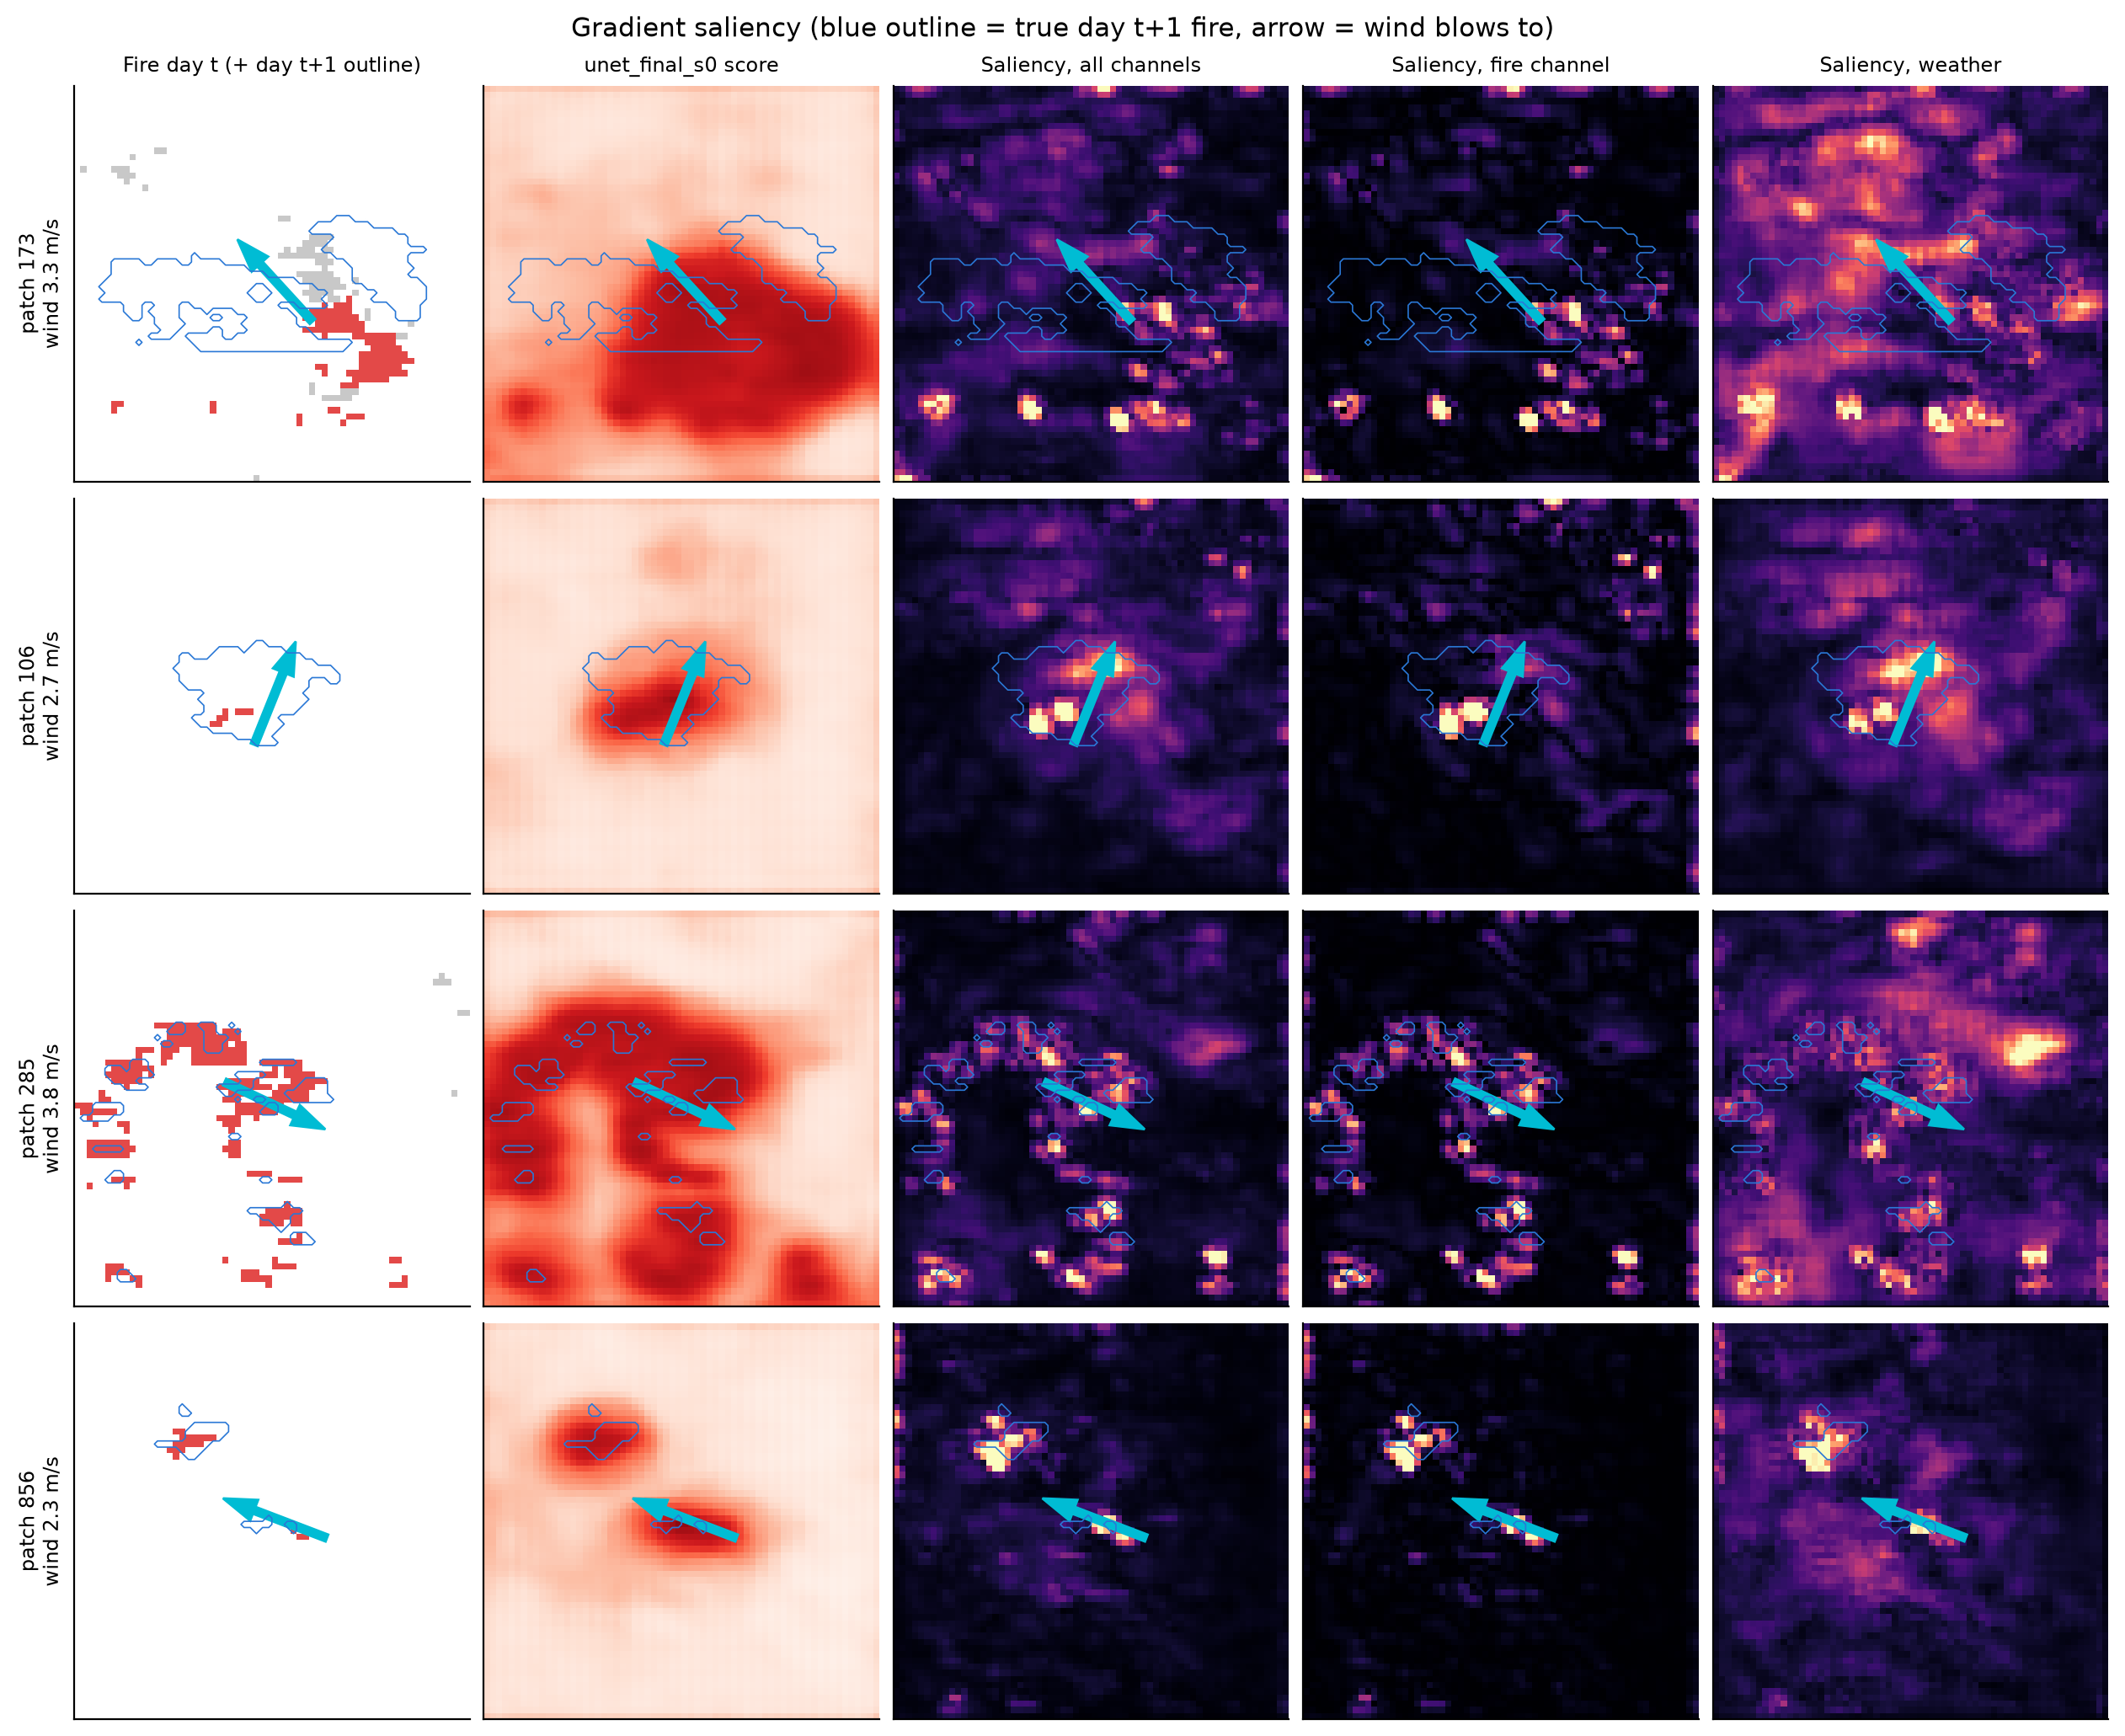
\includegraphics[height=0.70\textheight]{dl_eval_saliency_maps.png}
\end{columns}
\src{Gradient of each patch's predicted fire w.r.t. the inputs (final U-Net, seed 0). Notebook 03, sections 6 and 7.}
\end{frame}
